\documentclass[runningheads,a4paper,fleqn]{llncs}

\usepackage{url}
\usepackage{amsmath}
\usepackage{amssymb}
\usepackage{alltt}
\usepackage{lineno}
\usepackage{graphicx}
\usepackage[normalem]{ulem}

\usepackage{tikz}
\usetikzlibrary{arrows,petri,topaths}
\usepackage{tkz-berge}

\begin{document}

\title{Multi-Lane FlowPools: A detailed look}
\author{Tobias Schlatter\inst{1} \and Aleksandar Prokopec\inst{2} \and
  Heather Miller\inst{2} \and Philipp Haller\inst{2} \and Martin
  Odersky\inst{2}}

\authorrunning{Tobias Schlatter}

\institute{Student, EPFL \and Advisors, EPFL}

\maketitle

\begin{abstract}
  FlowPools, proposed by \cite{FP12} are a powerful way to express
  dataflow logic in highly parallelized applications. The original
  paper proposes two ways of implementing a FlowPool: Single-Lane
  FlowPools (SLFP) and Multi-Lane FlowPools (MLFP). While SLFPs 
  showed decent performance overall, insertion operations do not
  scale. MLFPs solve this limitation as benchmarks discussed in
  \cite{FP12} have shown. This report goes into the details of the
  implementation of MLFPs and lies out the benchmarking results from
  \cite{FP12} to show that MLFPs may reduce insertion time by $49 -
  54\%$ on a 4-core i7 machine with respect to comparable concurrent
  queue data structures in the Java standard library.
\end{abstract}

\section{Introduction}
The goal of this section is to briefly remind the reader of the
semantics and programming interface of a FlowPool and the basic ideas
behind the implementation of SLFPs to allow for better understanding
of the implementation of MLFPs.

\subsection{Programming Model}
The following operations are supported by a FlowPool. For a proof of
determinism, refer to \cite{FP12}.

\textbf{Append (\texttt{<<})} Inserts an element in the
FlowPool. Fails if the number of elements the FlowPool has been sealed
with is reached.\\
Signature: \verb+def <<(x: T): Unit+

\textbf{Foreach} Traverse elements in the FlowPool. Calls a closure
\verb+f+ exactly once (asynchronously) for each element added to the
FlowPool (until it is sealed). Returns future of number of elements in
pool. Foreach is normally implemented using the more general primitive
\verb+aggregate+.\\
Signature: \verb+def foreach[U](f: T => U):+ \verb+Future[Int]+

\textbf{Aggregate} Reduce elements in the FlowPool to a single
value. Starts off with \verb+zero+ as initial value to aggregate on,
calls \verb+op+ exactly once per element to add it to an aggregation,
finally uses \verb+cb+ to combine multiple aggregations into a single
one. Note that \verb+op+ is guaranteed to be executed only once per
element, whereas \verb+cb+ may be called any number of times\\
Signature: \verb+def aggregate[S]+\verb+(zero: =>S)+
\verb+(cb: (S, S) => S)+\\
\verb+(op: (S, T) => S):+ \verb+Future[S]+

\textbf{Builders} Abstraction to allow garbage collection of elements
that are no longer required. Allows insertion without reference to
initial pool (and hence all elements). See \cite{FP12} for details.

\textbf{Seal} Fixes the number of elements that will eventually be in
the pool allowing callbacks to be freed once reached. The final size
of the pool is required as argument in order to preserve the
determinism of the model. Subsequent call to \verb+seal+ will fail iff
the FlowPool has already been sealed with a different size or the
number of elements in the FlowPool is larger than the seal size.\\
Signature: \verb+def seal(size: Int): Unit+

Figure~\ref{fig:mon-impl} shows the implementation of some common
monadic operations on top of the given primitives.
\begin{figure}
\begin{minipage}[t]{4 cm}
\begin{alltt}
{\scriptsize
def filter
  (pred: T => Boolean)
  val p = new FlowPool[T]
  val b = p.builder
  aggregate(0)(_ + _) \{
    (acc, x) => if pred(x) \{
      b << x
      1
    \} else 0
  \} map \{ sz => b.seal(sz) \}
  p



}
\end{alltt}
\end{minipage}\begin{minipage}[t]{4 cm}
\begin{alltt}
{\scriptsize
def flatMap[S]
  (f: T => FlowPool[S])
  val p = new FlowPool[S]
  val b = p.builder
  aggregate(future(0))(add) \{
    (af, x) =>
    val sf = for (y <- f(x))
      b << y
    add(af, sf)
  \} map \{ sz => b.seal(sz) \}
  p

def add(f: Future[Int], g: Future[Int]) =
  for (a <- f; b <- g) yield a + b
}
\end{alltt}
\end{minipage}
\begin{minipage}[t]{4 cm}
\begin{alltt}
{\scriptsize
def union[T]
  (that: FlowPool[T])
  val p = new FlowPool[T]
  val b = p.builder
  val f = for (x <- this) b << x
  val g = for (y <- that) b << y
  for (s1 <- f; s2 <- g)
    b.seal(s1 + s2)
  p
}
\end{alltt}
\end{minipage}

\caption{Some common monadic operations implemented using the FlowPool
  primitives (taken from \cite{FP12})} \label{fig:mon-impl}
\end{figure}


\subsection{Single-Lane FlowPool}
SLFPs are implemented using a single linked-list of arrays of
elements, where the last non-empty element does not hold actual data,
but the state of the FlowPool, i.e. a list with all the callbacks and
the seal state of the FlowPool. Changes to the SLFP are only allowed
by CASing at this particular point, which hence serves as
linearization point of the data structure.

With competing, concurrent writers, this approach does not scale
nicely (see figure~\ref{fig:eval-cpu-scaling}). Mainly due to cache
contention (multiple CPUs often write to close memory locations) and
CAS collisions.

\section{Implementation}
MLFPs take advantage of the lack of ordering guarantees in the
FlowPool semantics to remove the limitation of SLFPs with respect to
scaling by applying a simple but effective idea: Instead of having a
single SLFP, we use one SLFP (from now on called lane) for each
processor (or thread). This means, that on one hand, every processor
(or thread) gets its own lane to which it appends elements to,
avoiding CAS collisions and cache contention. On the other hand, every
callback or aggregation has to be registered on each of these lanes
separately and completing the callback future has to be externally
synchronized.

In the following, the implementation of the FlowPool operations in the
MLFP are explained in detail. Please refer to
figure~\ref{fig:mlfp-pseudocode} for pseudo code of the operations.

\subsection{Callbacks}
When calling \verb+aggregate+ on a MLFP, the implementation has to
ensure that a copy of this callback is known to every underlying lane
and that upon completion of the callbacks for every lane, the values
are aggregated in the final result and the future is completed. Note
that callback addition to a given lane is no different than in SLFPs.

The aggregation of each lane's final values is done using a FlowLatch,
a construct that allows aggregating a given number of values into a
single one using similar semantics as a FlowPool. A FlowLatch may
supply a future that is completed with the aggregated value, once the
expected number of values has been supplied. \verb+aggregate+ returns
this future to the caller.

\subsection{Seal}
The \verb+seal+ operation is the only one whose complexity increases
with multiple lanes, as the overall size guarantee has to be
established over all lanes while preserving lock-freedom and
linearizability, especially in the face of errors occurring while
sealing.

To ensure the latter, a global seal state (stored in a location common
to the whole MLFP) is required. The global seal may be in one of the
following states (state transition graph in
figure~\ref{fig:seal-states}):
\begin{itemize}
\item \verb+Unsealed+ (U): No seal has yet been attempted, or all
  seals have failed.
\item \verb+Proposition(size)+ (P): Sealing with given (total) size is
  being attempted. No other sealing operation may be attempted until
  this state is resolved to one of the other two. Threads attempting
  to seal and encountering a \verb+Proposition+ state, shall help the
  resolution of the state. (This is required to ensure lock-freedom)
\item \verb+Sealed(size, remain)+ (S): The MLFP has been sealed with
  size \verb+size+, where at the moment of the sealing, \verb+remain+
  free slots were remaining. The latter value is required to
  distribute the remaining element slots amongst the lanes and will be
  explained in detail later.
\end{itemize}

%% Seal-State transition graph
\begin{figure}
  \centering
  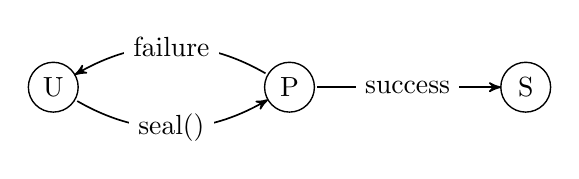
\begin{tikzpicture}[ node distance = 2cm ]
    \Vertex[x = 0, y = 0]{U}
    \Vertex[x = 3, y = 0]{P}
    \Vertex[x = 6, y = 0]{S}

    \tikzset{EdgeStyle/.style={post}}       % directed edges

    \Edge[label = success](P)(S)

    \tikzset{EdgeStyle/.append style = {bend right}}
    \Edge[label = {seal()}](U)(P)
    \Edge[label = failure](P)(U)

  \end{tikzpicture}
  \caption{State-transition graph of MLFP seal state}
  \label{fig:seal-states}
\end{figure}

Further, each lane holds its own seal state (similar to SLFPs) which
may be one of the following. The state transitions are the same as for
the global state (figure~\ref{fig:seal-states}).
\begin{itemize}
\item \verb+CallbackList+ (U): The lane is unsealed. A seal procedure
  might have been started but is not yet completed. Insertion may be
  handled as in a SLFP.
\item \verb+SealTag+ (P): A seal procedure has been started and any
  writer should resolve the tag by either helping to finish the
  sealing or replace it based on the global state.
\item \verb+Seal(size)+ (S): This lane has been sealed with the given 
  size.
\end{itemize}

In the following, the different parts of the sealing procedure are
explained in detail.

\textbf{Seal} When a thread calls \verb+seal()+ it first checks the
current state of the MLFP. If it is in unsealed state, it tries to
change the seal state to proposition and then continue with the
sealing. If the MLFP is already in proposition state, it helps
to complete the current seal. If the MLFP is in \verb+Sealed+ state, the
call returns immediately, succeeding if the size in \verb+Sealed+ is
equal to the proposed sealing size, failing otherwise.

\textbf{Help Sealing} Once the MLFP is in proposition state, any
thread attempting to seal (or inserting an element as we will see
later), will start propagating the proposition state to each lane. It
does this by placing the special token \verb+SealTag+ into the state
location of the given lane, using a procedure similar to \verb+seal()+
on SLFPs.

A thread that tries to insert an element and encounters a
\verb+SealTag+ must resolve the tag before it can continue on
(explained later). This ensures that, once a \verb+SealTag+ has been
placed in a lane, its size does not change any more until the seal is
finished, which allows to calculate a snapshot of the total number of
elements in the MLFP. Note that during this procedure, one might also
find that the seal has been completed (when encountering a \verb+Seal+
in a lane). In such a case, the helping can be stopped prematurely.

Note that each \verb+SealTag+ holds a reference to the global
proposition object that caused its creation. This is required as a
sentinel as other seal tags might still be present from a failed
attempt to seal.

When a thread that succeeds in calculating the snapshot of the size,
it will then try to change the MLFP's state to sealed (or to unsealed,
if the number of elements is too big) and replace every occurrence of
\verb+SealTag+ in the lanes by a \verb+Seal+.

\textbf{Resolution of seal tags} When a writer encounters a
\verb+SealTag+ it first checks the current global state. If it
indicates, that the seal operation corresponding to the \verb+SealTag+
is still going on, the writer helps sealing as described above, then
retries writing. If the global state indicates that the structure has
been sealed, the writer calculates the remaining slots for this lane
according to the following formula and then seals this lane.
\[ n_{seal} = n_{cur} + \frac{n_{remain}}{l_{total}} +
   1_{\{ l_{cur} < n_{remain} \bmod l_{total} \}} \]
If the writer finds that the current global state is unsealed or a
different proposition than in the tag, it removes the tag and
continues inserting normally.

\textbf{Finalization} Some procedures that are required to invoke the
callback scheduling properly when sealing (i.e. ensuring the
finalization procedure of each callback is called exactly once) have
been omitted here for simplicity.

\subsection{Insertion}
Insertion into a MLFP happens the same way as into a SLFP, however,
the lane in which the element is to be inserted has to be chosen
first. For the choice of the lane we want to:
\begin{itemize}
\item Avoid collision between competing threads to a maximum.
\item Allow to change the thread-lane assignment, once some lanes have
  been entirely filled (after a seal).
\item Assure we can properly fill up the FlowPool entirely.
\end{itemize}
To achieve this, the following mapping is used at the beginning:
\[ l_{cur} = T_{cur} \bmod l_{total} \qquad
  (T_{cur} \text{ : Current thread ID}) \] 

When the first collision (i.e. attempted insertion into a full lane)
happens, the following hashed mapping is used \cite{BSH}:
\[ l_{cur} = \mathrm{rb}((T_{cur} + C) \cdot 9e3775cd_{16})
   \cdot 9e3775cd_{16}  \bmod l_{total} \]
where $C$ is the (global) number of collisions so far and
$\mathrm{rb}(\cdot)$ inverses the byte order.

After a certain number of collisions (currently the number of lanes),
the insertion switches to a linear search over all lanes to guarantee
that either the FlowPool is filled, or an error is raised due to too
many inserted elements.

Experimental results in figure~\ref{fig:lanef-scaling} show that there
is no use in having more than one lane per inserting thread and hence
that the upper lane selection strategy is efficient. For details,
refer to section~\ref{sec:evaluation}. 

\begin{figure}
  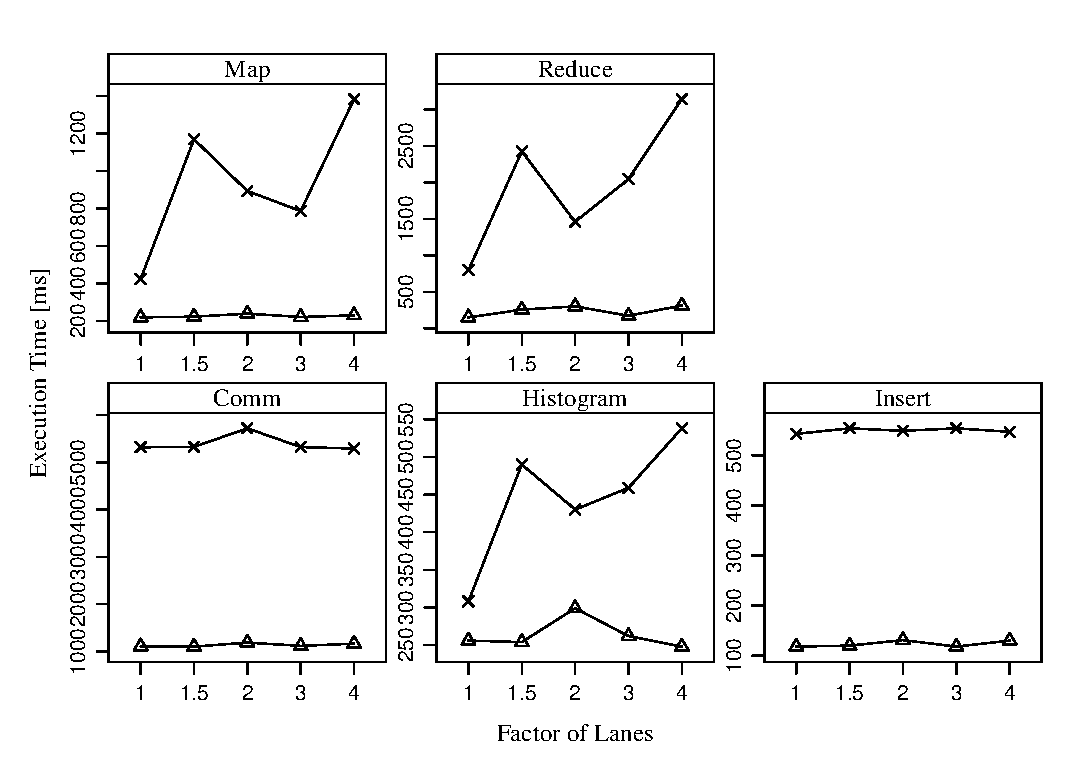
\includegraphics[width=\textwidth]{../../benchmarks/graphs/lanef-scaling}
  \caption{Execution times with respect to number of lanes per
    inserting thread in MLFPs. $\times$~UltraSPARC~T2,
    $\triangle$~4-core~i7}
  \label{fig:lanef-scaling}
\end{figure}

\begin{figure}

\centering

\begin{minipage}[b]{6cm}
\begin{alltt}
{\scriptsize
{\internallinenumbers{def aggregate[S](zero: =>S)
                (cmb: (S, S) => S)
                (folder: (S, T) => S):
    Future[S] = \{

  val aggregator = FlowLatch[S](zero)(cmb)
  aggregator.seal(laneCount)
    
  for (l <- lanes) \{
    l.registerCB(folder, zero, aggregator)
  \}
  
  aggregator.future
\}

def seal(size: Int) \{
  val cur_state = state
  cur_state match \{
    case Unsealed =>
      val ns = Proposition(size)
      if (!CAS(state, cur_state, ns))
        seal(size)
      else if (!helpSeal(ns)) failure()
    case p: Proposition =>
      if (helpSeal(p)) failure()
      else seal(size)
    case Sealed(sz,_) if size != sz =>
      failure("already sealed")
    case _ => // Done
  \}
\}

def tryResolveTag[T](t: SealTag[T]) \{
  cur_state match \{
    case p: Proposition if (p eq t.p) =>
      helpSeal(p)
    case Sealed(_,rem) =>
      val sz = sealSize(cur_state)
      writeSeal(Seal(sz))
    case _ => revertTag()
  \}
\}
}}}
\end{alltt}
\end{minipage}
\begin{minipage}[b]{6cm}
\begin{alltt}
{\scriptsize
{\internallinenumbers{def helpSeal(p: Proposition): Boolean = \{
  var sizes: Int = 0

  for (l <- lanes) \{
    writeSealTag(l, p) match \{
      case OnGoing(v)   =>
        sizes = sizes + v
      case Finished(success) => return success
    \}
  \}

  if (sizes <= p.size) \{
    // Seal MUST succeed
    val remaining = p.size - sizes
    val ns = Sealed(p.size, remaining)
    if (CAS(state, p, ns))
      finalizeSeals(remaining)
    true
  \} else \{
    // Seal MUST fail
    CAS(state, p, Unsealed)
    false
  \}

\}

def append(x: T) \{
  val index = \{
    if (collisions <= 0)
      curTID % laneCount
    else if (collisions <= laneCount)
      hash(curTID, collisions)
    else
      findEmptyLane() // Fails if not found
  \}

  if (!lanes(index).append(x)) \{
    increment(collisions)
    append(x)
  \}

\}
}}}
\end{alltt}
\end{minipage}

\caption{Multi-Lane FlowPool operations pseudo code}
\label{fig:mlfp-pseudocode}

\end{figure}

\section{Evaluation}
\label{sec:evaluation}
This section comes mainly from~\cite{FP12} and is just repeated here
for convenience.

\textbf{Setup} We evaluate our implementation (single-lane and
multi-lane FlowPools) against the LinkedTransferQueue
\cite{SchererLS09} for all benchmarks and the ConcurrentLinkedQueue
\cite{Michael96} for the insert benchmark, both found in JDK 1.7, on
three different architectures; a quad-core 3.4 GHz i7-2600, 4x
octa-core 2.27 GHz Intel Xeon x7560 (both with hyperthreading) and an
octa-core  1.2GHz UltraSPARC T2 with 64 hardware threads. 

\textbf{Benchmarks and Scaling} In the \emph{Insert} benchmark, Figure
\ref{fig:eval-cpu-scaling}, we evaluate the ability to write
concurrently, by distributing the work of inserting $N$ elements into
the data structure concurrently across $P$ threads. 
In Figure \ref{fig:eval-cpu-scaling}, it's evident that both
single-lane FlowPools and concurrent queues do 
not scale well with the number of concurrent threads, particularly
on the i7 architecture. They seem to slow down rapidly, likely due to cache
line collisions and CAS failures.
On the other hand, multi-lane FlowPools scale well, as threads
write to different lanes, and hence different cache lines on
most occasions, meanwhile also avoiding CAS failures. This may reduce execution
time for insertions up to $54\%$ on the i7, $63\%$ on the
Xeon and $92\%$ on the UltraSPARC T2.

Usage of the inserted data is evaluated in the \emph{Reduce}, \emph{Map} (both
in Figure \ref{fig:eval-cpu-scaling}) and \emph{Histogram} benchmarks (Figure
\ref{fig:eval-hist-comm}). It's important to note that the \emph{Histogram} benchmark
serves as a ``real life'' example, which uses both the \verb=map= and \verb=reduce=
operations that are benchmarked in Figure \ref{fig:eval-cpu-scaling}.

The \textit{Reduce} benchmark starts $P$ threads which concurrently
insert a total of $N$ elements. The \verb=aggregate= operation is used
to reduce the set of values inserted into the pool. Note that in the
FlowPool implementation there may be as many threads computing the
aggregation as there are different lanes -- elements from different
lanes are batched together once the pool is sealed.

The \textit{Map} benchmark is similar to the \textit{Reduce}
benchmark, but instead of reducing a value, each element is mapped
into a new one and added to a second pool.

In the \textit{Histogram} benchmark, Figure \ref{fig:eval-hist-comm},
$P$ threads produce a total of $N$ elements, adding them to the
FlowPool. The \verb=aggregate= operation is then used to produce 10
different histograms concurrently with a different number of bins. 
Each separate histogram is constructed by its own thread (or up to
$P$, for multi-lane FlowPools).
A crucial difference between queues and FlowPools here, is that with 
FlowPools, multiple histograms are produced 
by invoking several \verb=aggregate= operations, while queues require
writing each element to several queues-- one for each histogram.
Without additional synchronization, reading a single queue is not an
option, since elements have to be removed from the queue eventually, and
it is not clear to each reader when to do this.
With FlowPools, elements are automatically garbage collected when no
longer needed.

Finally, to validate the last claim of garbage being automatically
collected, in the \textit{Communication/Garbage Collection} benchmark, 
Figure \ref{fig:eval-hist-comm}, we create a pool in which a
large number of elements $N$ are added concurrently by $P$
threads. Each element is then processed by one of $P$ threads through
the use of the \verb=aggregate= operation.
We benchmark against linked transfer queues, where $P$ threads concurrently remove
elements from the queue and process it.
For each run, we vary the size of the $N$ and examine its impact on the execution time.
Especially in the cases of the Intel architectures, the multi-lane 
FlowPools perform considerably better than the linked transfer queues. 
As a matter of fact, the linked transfer queue on the Xeon benchmark ran out of 
memory, and was unable to complete, while the multi-lane FlowPool scaled effortlessly 
to 400 million elements, indicating that unneeded elements are properly garbage collected.

\textbf{Scaling in Input Size} In figure~\ref{fig:eval-size-scaling}
we can see that the Input, Map, Reduce and Histogram benchmark all
scale linearly in the input size with any parallelism level. The Comm
benchmark has not been tested for different sizes. 

\textbf{Multi-Lane Scaling} By default, the number of lanes is set to
the parallelism level $P$, corresponding to the number of used
CPUs. However, since the implementation has to use hashing on the
thread IDs instead of the real CPU index, we tested whether varying
the number of lanes to $1.5 P$, $2P$, $3P$ and $4P$ results in
performance gain due to fewer collisions. Benchmarks have shown (see
figure~\ref{fig:lanef-scaling}) that this yields no observable gain --
in fact, this sometimes even decreased performance slightly.

\textbf{Performance Gain} As stated in the abstract, FlowPools -- or
more precisely multi-lane FlowPools -- may reduce execution time by
$49 - 54\%$ on 4-core i7. These figures have been obtained by
comparing medians of execution times for insertions between multi-lane
FlowPools and concurrent linked queues (which were always faster than 
linked transfer queues), where each structure was evaluated on its
optimal parallelization level. The resulting data is shown in
table~\ref{tbl:execution-times}.

\textbf{Methodology} All the presented configurations have been
measured $20$ times, where the $5$ first values have been discarded to
let the JIT stabilize. Aggregated values are always medians. The
benchmarks have been written using \verb=scala.testing.Benchmark= and
executed through SBT\footnote{Simple Build Tool} using the following
flags for the JavaVM: \texttt{-Xmx2048m -Xms2048m -XX:+UseCondCardMark
  -verbose:gc -XX:+PrintGCDetails -server}.

\begin{figure}
\centering
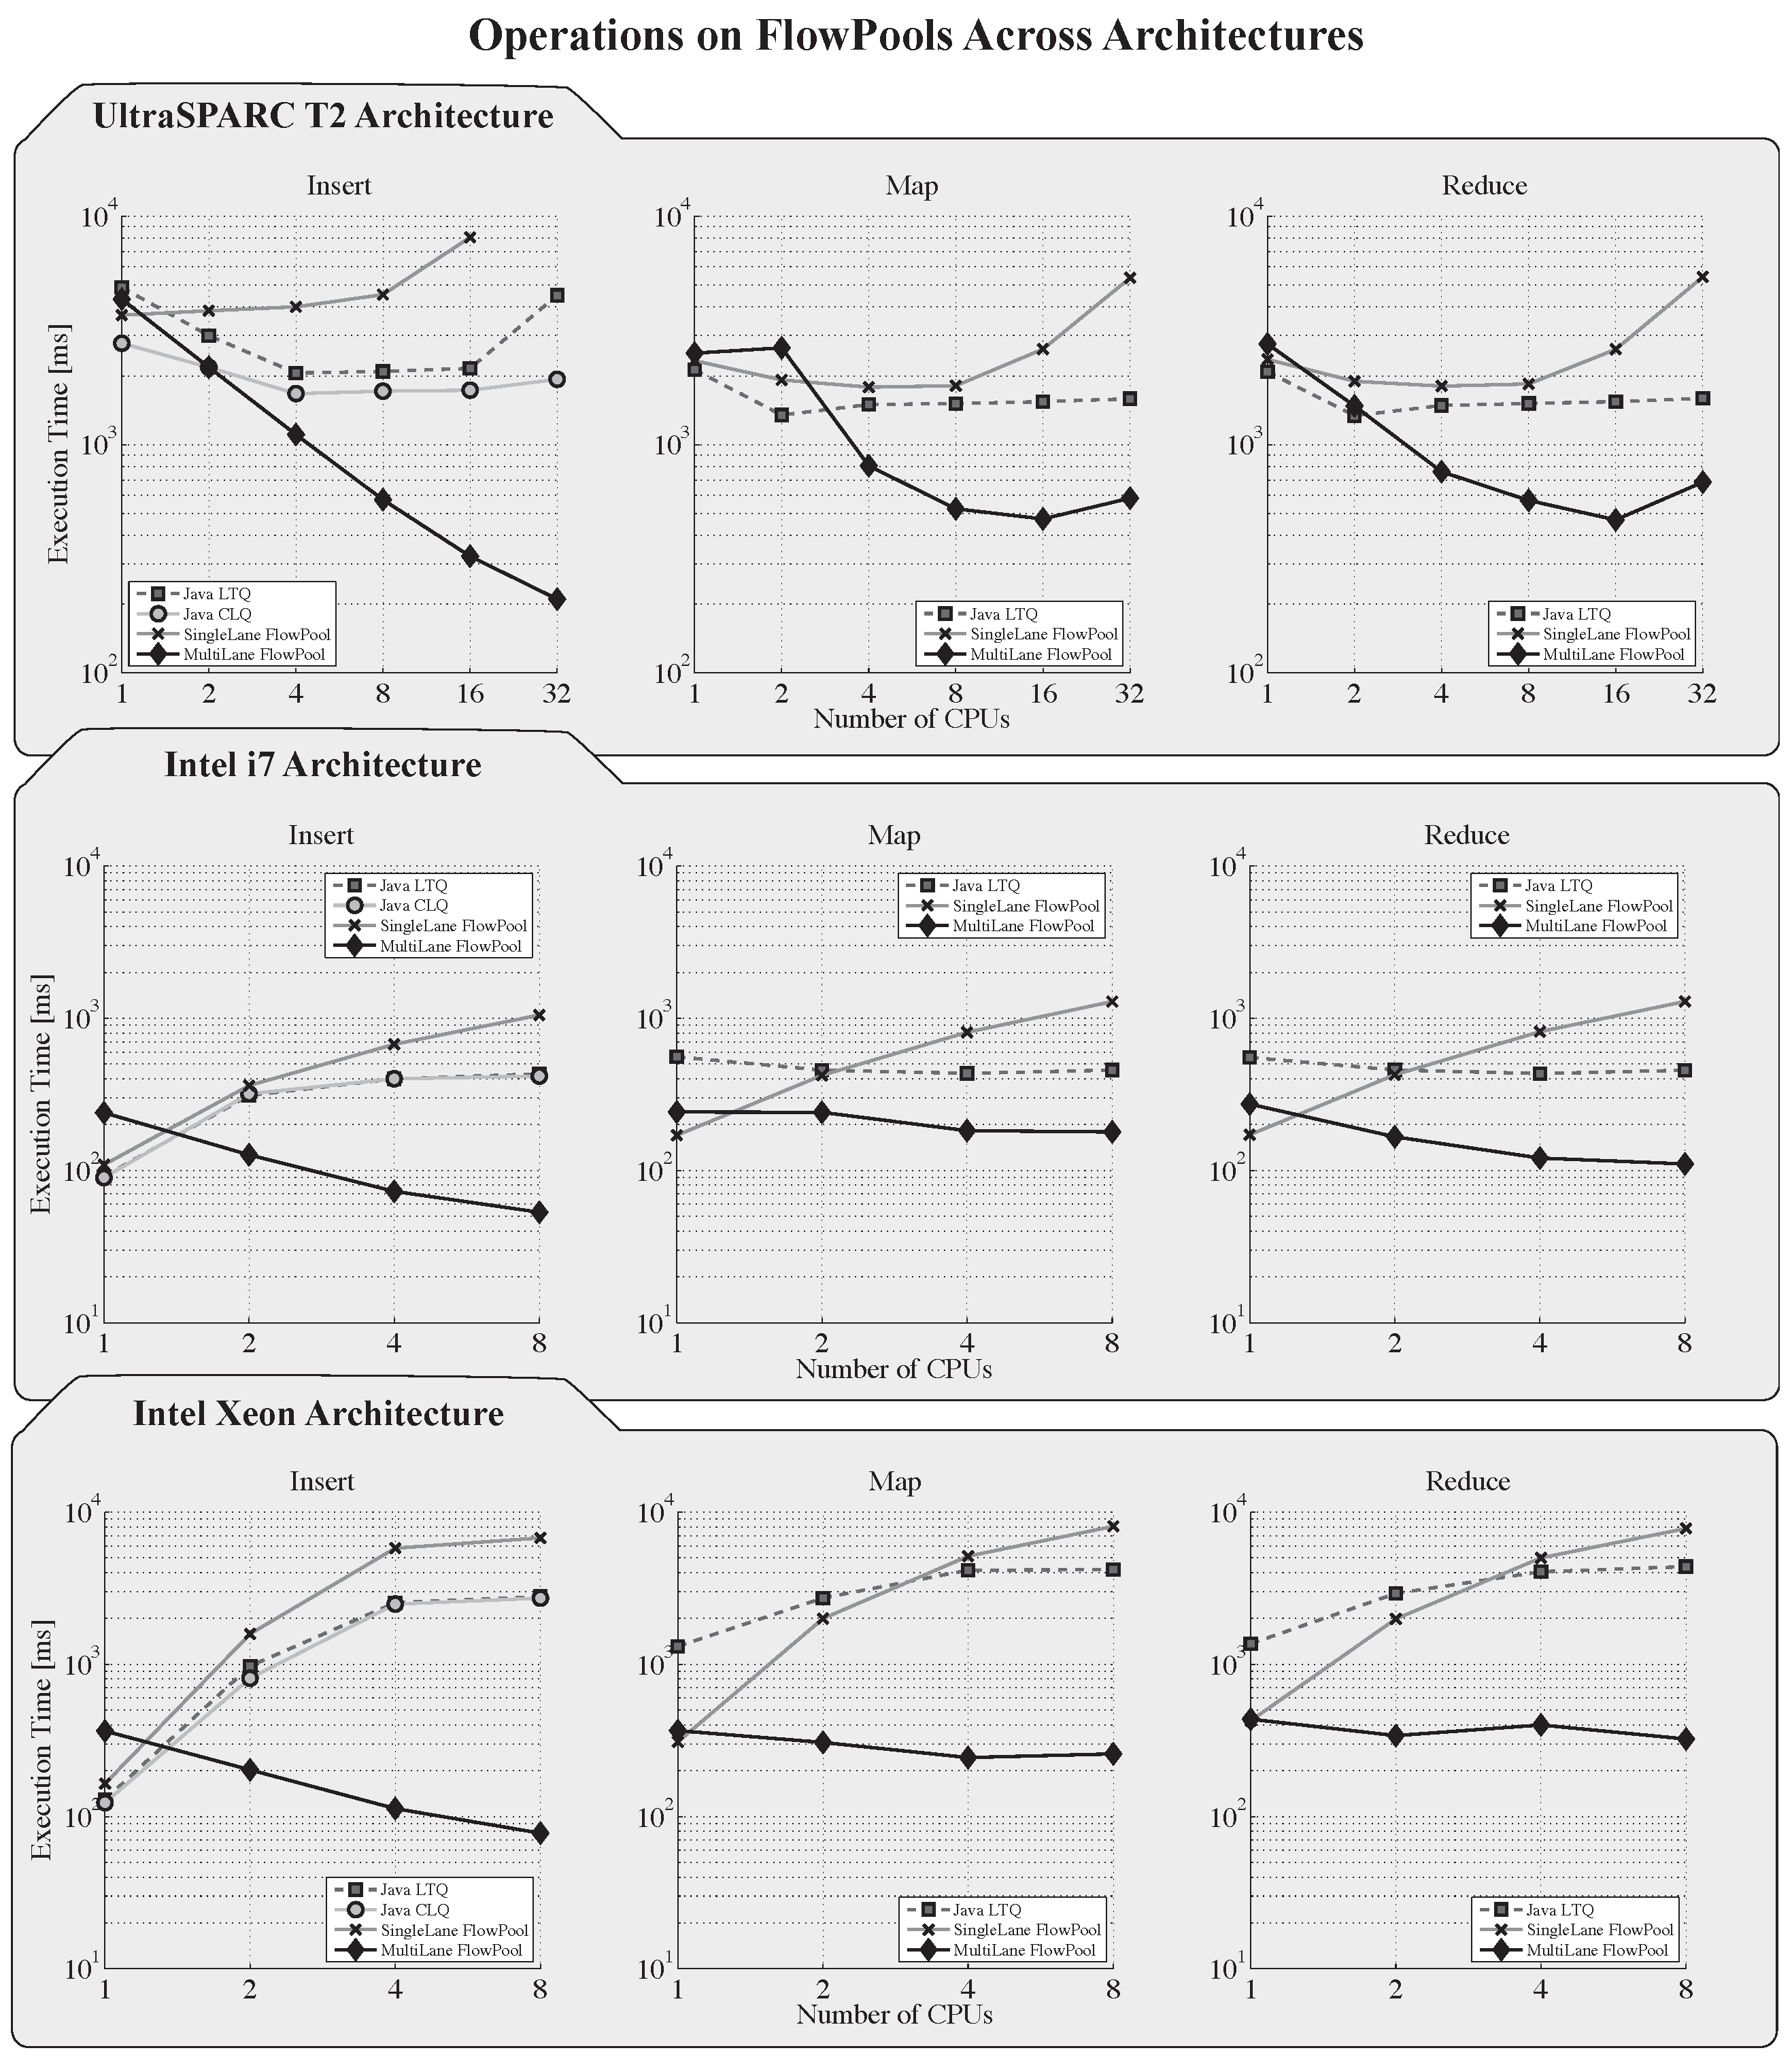
\includegraphics[width=\textwidth]{../../benchmarks/graphs/scaling-operations}
\caption{Execution time vs parallelization across three different
  architectures on three important FlowPool operations; insert, map,
  reduce.}
\label{fig:eval-cpu-scaling}
\end{figure}

\begin{figure}
\centering
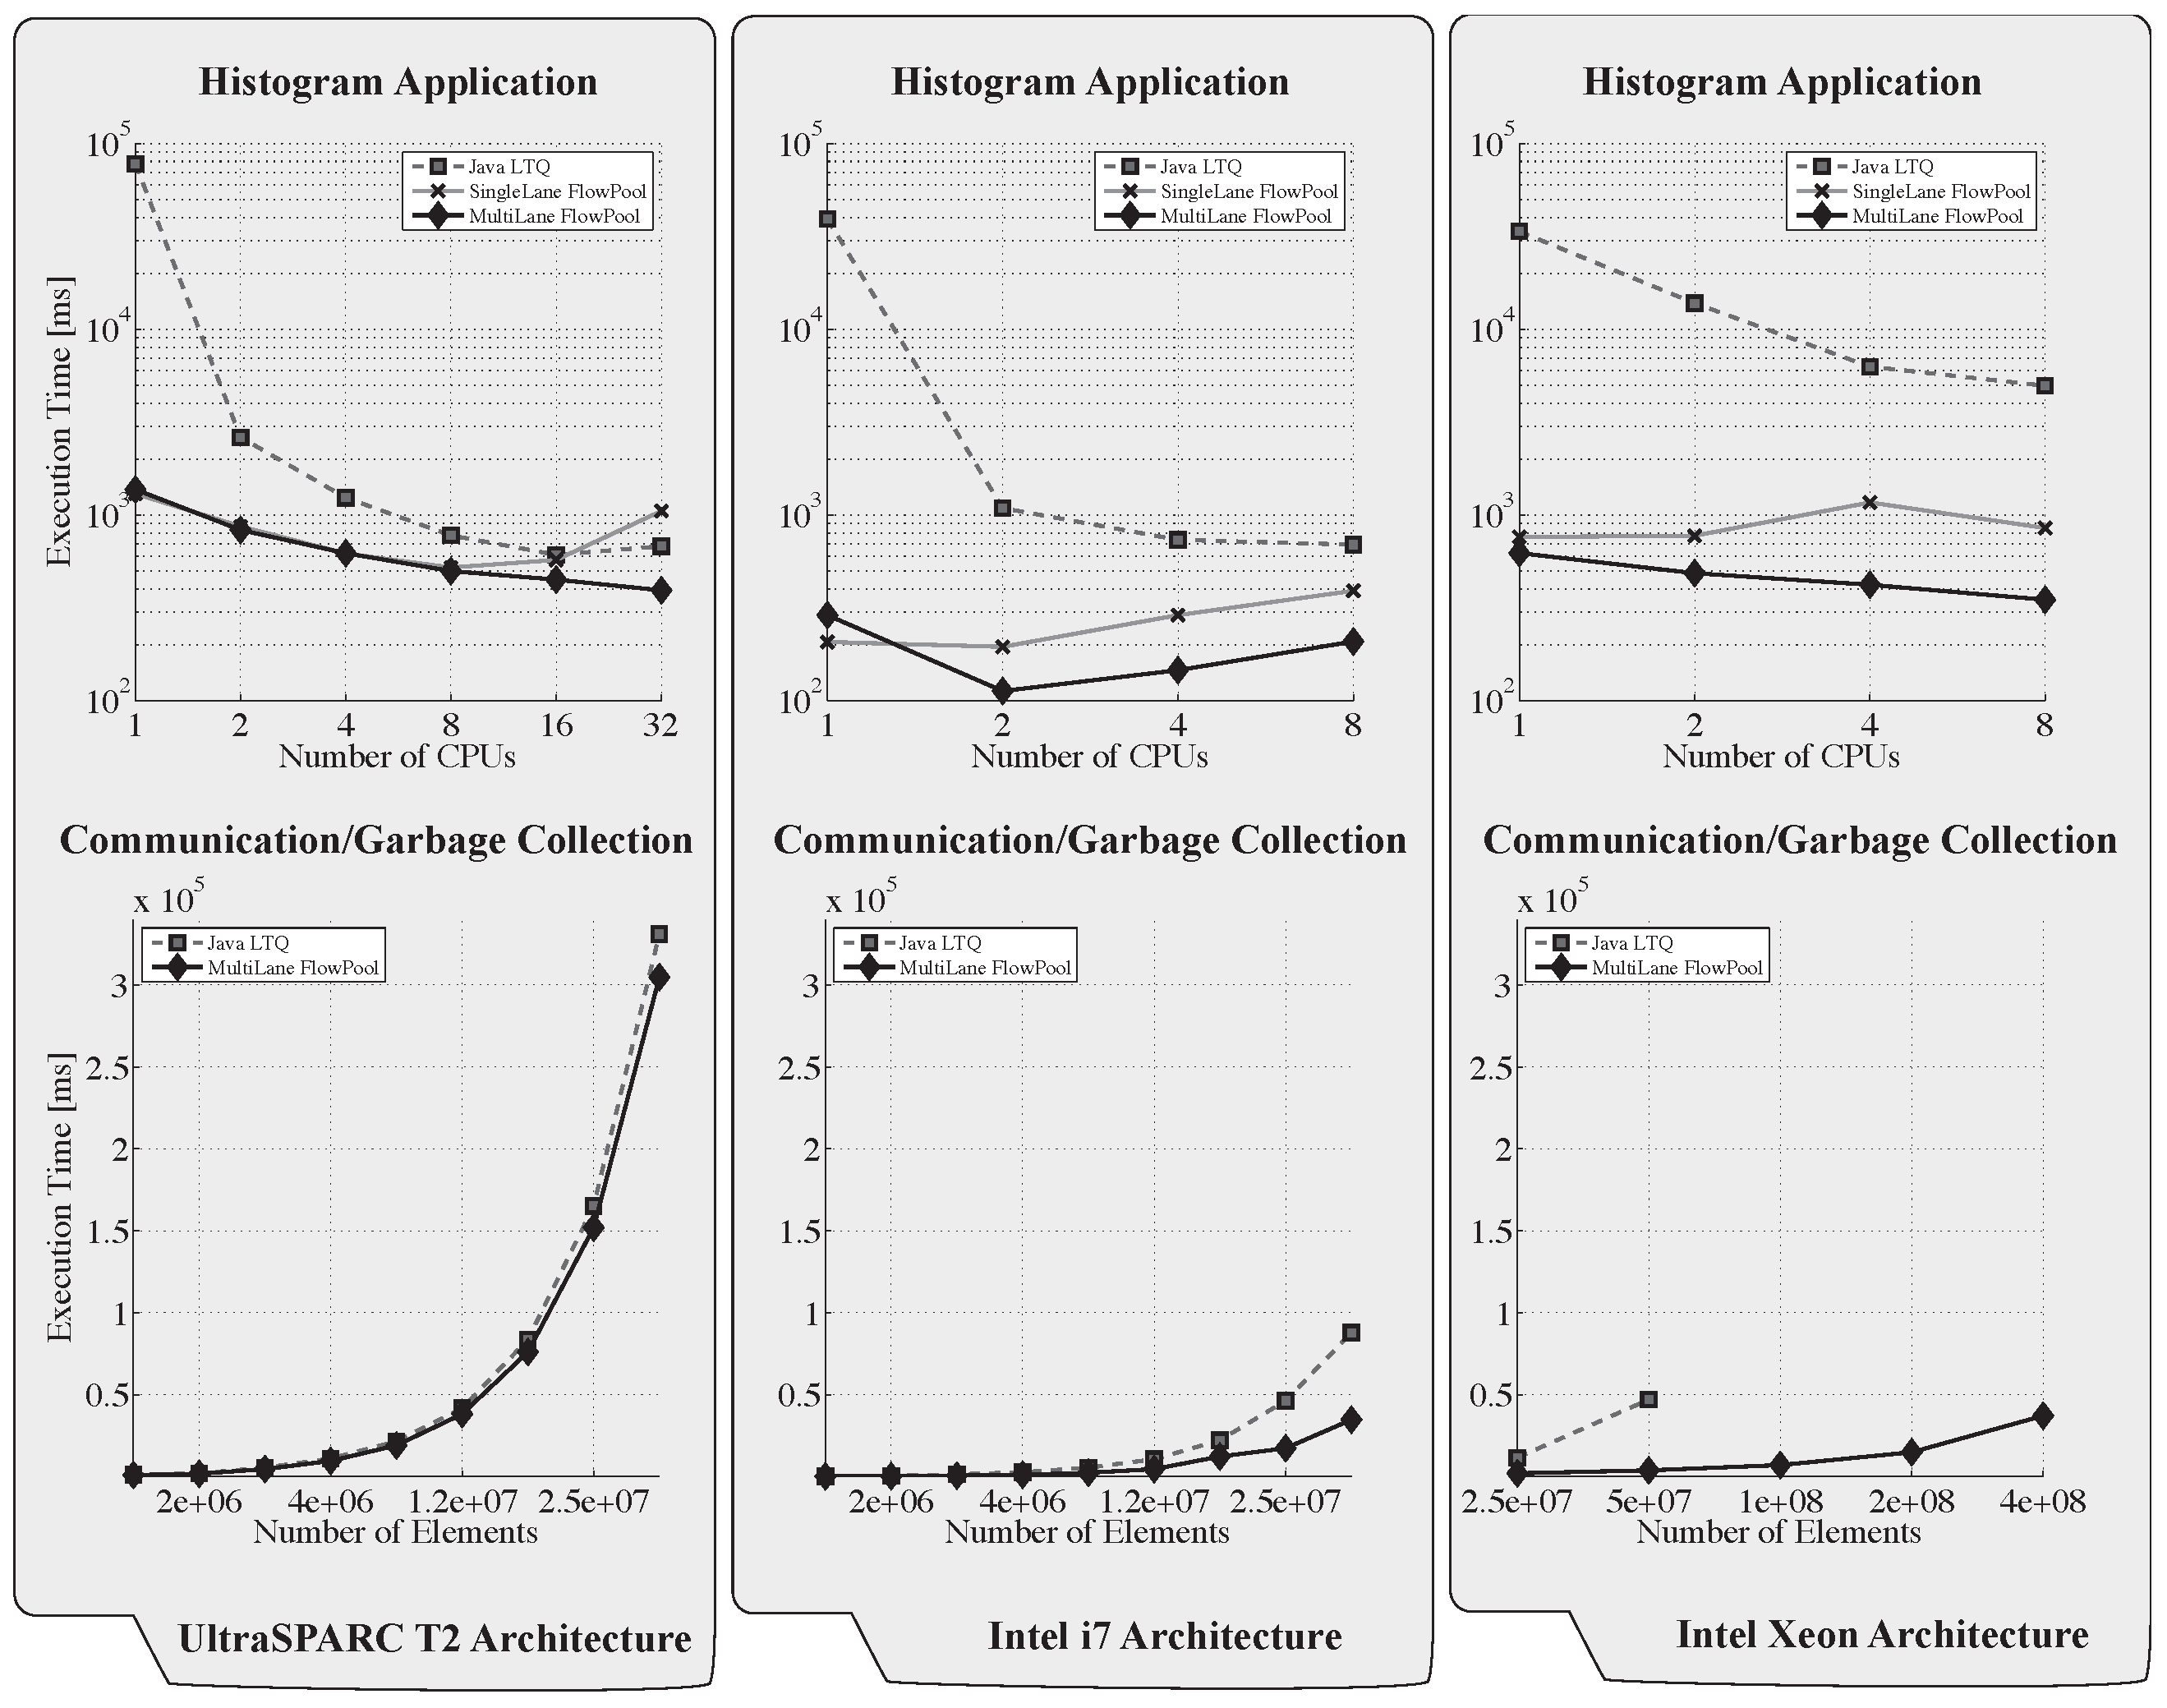
\includegraphics[width=\textwidth]{../../benchmarks/graphs/hist-comm}
\caption{Execution time vs parallelization on a real histogram application
(top), \& communication benchmark (bottom) showing memory efficiency, 
across all architectures.}
\label{fig:eval-hist-comm}
\end{figure}

\begin{figure}
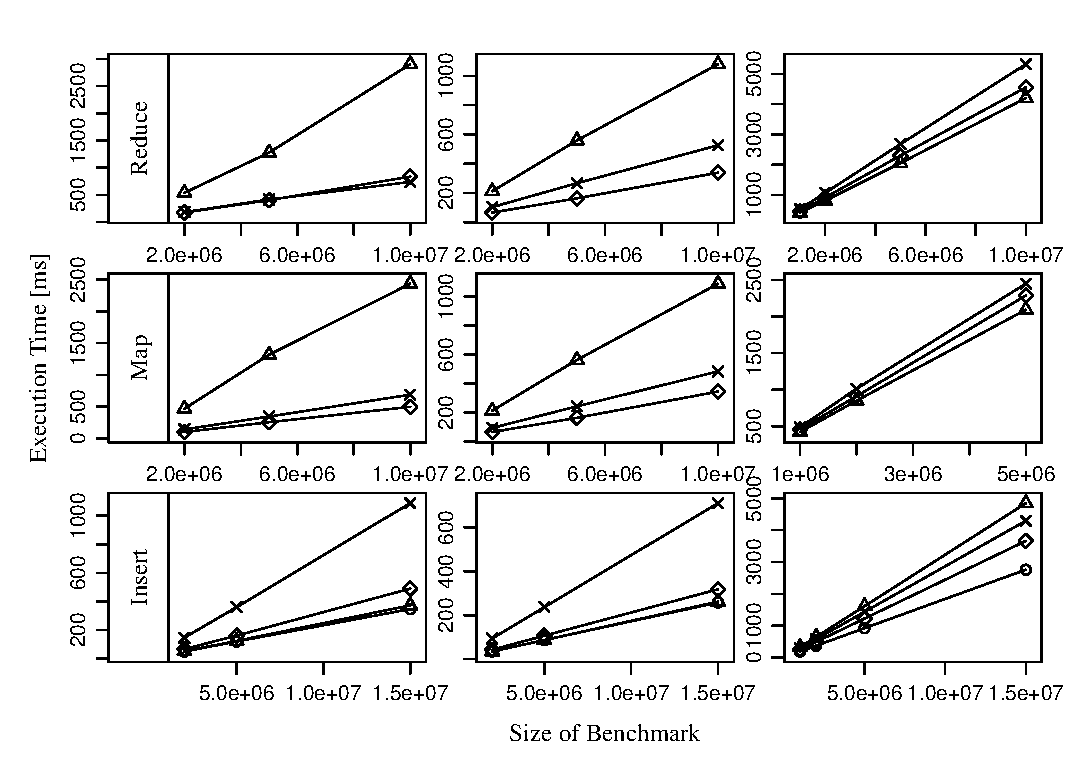
\includegraphics[width=\textwidth]{../../benchmarks/graphs/size-scaling-par1}
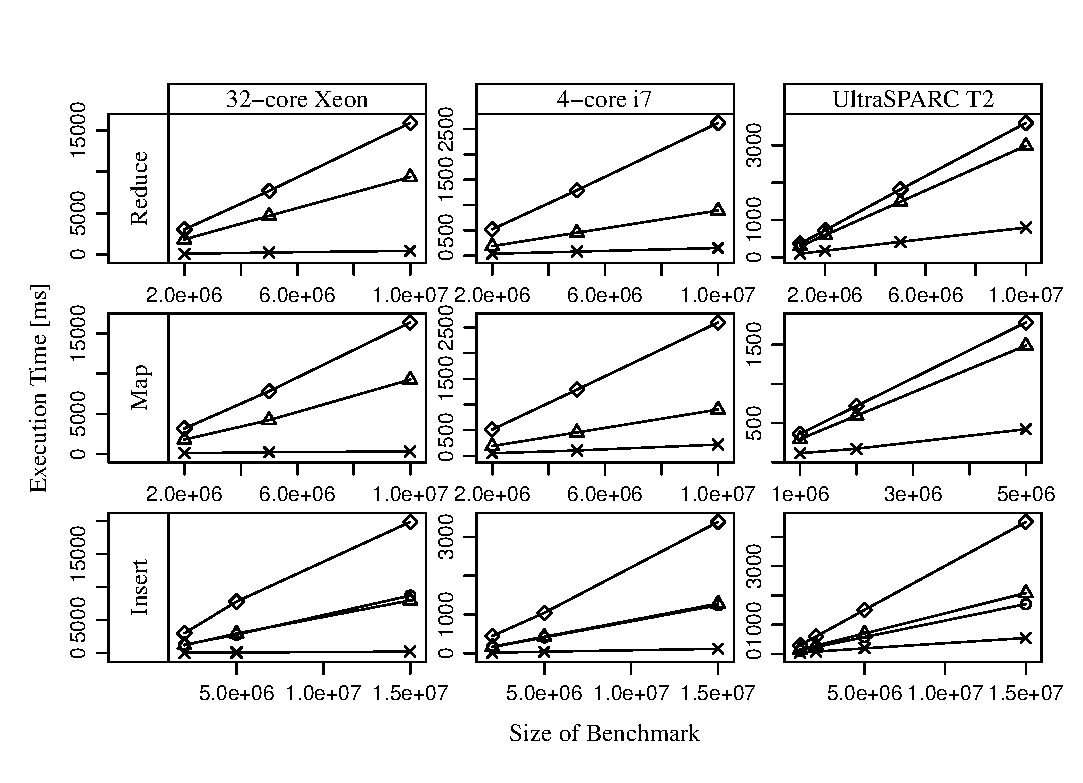
\includegraphics[width=\textwidth]{../../benchmarks/graphs/size-scaling-par8}
\caption{Execution time vs benchmark size ($P = 1, 8$).
  $\Diamond$ SLFP,
  $\times$ MLFP,
  $\triangle$ linked transfer queue,
  $\circ$ concurrent linked queue} \label{fig:eval-size-scaling}
\end{figure}

\begin{table}[t]
\centering
\begin{tabular}{l@{\qquad}r@{\quad}r@{\quad}r@{\quad}r@{\quad}r@{\qquad}r}
  Architecture & Elements & FlowPool $t [ms]$ & $P$ & Queue $t [ms]$ & $P$ & decr.\\
\hline
    4-core i7 &  2M &  17 &  8 &   35 & 1 & 51\%\\
    4-core i7 &  5M &  44 &  8 &   87 & 1 & 49\%\\
    4-core i7 & 15M & 118 &  8 &  258 & 1 & 54\%\\
\hline
UltraSPARC T2 &  1M &  23 & 32 &  111 & 4 & 79\%\\
UltraSPARC T2 &  2M &  34 & 64 &  224 & 4 & 84\%\\
UltraSPARC T2 &  5M &  62 & 64 &  556 & 4 & 88\%\\
UltraSPARC T2 & 15M & 129 & 64 & 1661 & 4 & 92\%\\
\hline
 32-core Xeon &  2M &  30 &  8 &   50 & 1 & 40\%\\
 32-core Xeon &  5M &  46 & 64 &  120 & 1 & 61\%\\
 32-core Xeon & 15M & 126 & 64 &  347 & 1 & 63\%\\
\end{tabular}

\caption{Execution times for insert benchmark for MLFP and concurrent
  linked queues, including execution time decrease
  percentage.} \label{tbl:execution-times}
\end{table}

\section{Conclusion}
In this report we have shown that a FlowPool as proposed by
\cite{FP12} can be implemented in a scalable way by using multiple
single-lane FlowPools. Further, we have provided a detailed
description including pseudo-code of how a multi-lane FlowPool is
implemented, especially with respect to sealing -- which had to be
fundamentally changed -- and the lane assignment rehashing strategy,
that does not exist in single-lane FlowPools. We used and included
benchmark results from the original paper to show that MLFPs scale
nicely, may significantly reduce execution time with respect to
comparable data structures and that the proposed rehashing strategy is
efficient for a number of lanes equal to the number of inserting
threads.

\bibliographystyle{abbrv}
\bibliography{bib}

\end{document}

%%% Local Variables: 
%%% mode: latex
%%% TeX-master: t
%%% End: 
